  \documentclass[10pt,twocolumn,letterpaper]{article}

\usepackage{cvpr}
\usepackage{times}
\usepackage{epsfig}
\usepackage{graphicx}
\usepackage{amsmath}
\usepackage{amssymb}
\usepackage{algorithm}
\usepackage{algpseudocode}

% Include other packages here, before hyperref.

% If you comment hyperref and then uncomment it, you should delete
% egpaper.aux before re-running latex.  (Or just hit 'q' on the first latex
% run, let it finish, and you should be clear).
\usepackage[pagebackref=true,breaklinks=true,letterpaper=true,colorlinks,bookmarks=false,draft]{hyperref}


%%% comment \ShowNotes out to remove all colored comments defined with \newcommand below %%%
\newcommand*{\ShowNotes}{}

\ifdefined\ShowNotes
  \newcommand{\colornote}[3]{{\color{#1}\bf{#2: #3}\normalfont}}
\else
  \newcommand{\colornote}[3]{}
\fi
% maybe requires 
\usepackage[usenames]{color}
\definecolor{darkred}{rgb}{0.7,0.1,0.1}
\definecolor{darkmagenta}{rgb}{0.1,0.7,0.1}
\definecolor{cyan}{rgb}{0.7,0.0,0.7}
\definecolor{dblue}{rgb}{0.2,0.2,0.8}
\definecolor{maroon}{rgb}{0.76,.13,.28}
\definecolor{burntorange}{rgb}{0.81,.33,0}

%\newcommand {\note}[1]{\colornote{maroon}{Note}{#1}}
\newcommand {\todo}[1]{\colornote{cyan}{TODO}{#1}}
\newcommand {\lihi}[1]{\colornote{magenta}{LZ}{#1}}
\newcommand {\ayellet}[1]{\colornote{blue}{AT}{#1}}
\newcommand {\nadav}[1]{\colornote{red}{NA}{#1}}

% \cvprfinalcopy % *** Uncomment this line for the final submission

\def\cvprPaperID{****} % *** Enter the CVPR Paper ID here
\def\httilde{\mbox{\tt\raisebox{-.5ex}{\symbol{126}}}}

% Pages are numbered in submission mode, and unnumbered in camera-ready
\ifcvprfinal\pagestyle{empty}\fi
\begin{document}

%%%%%%%%% TITLE
\title{Partial Matching of 3D Shapes using Deformable Diversity}

\author{First Author\\
Institution1\\
Institution1 address\\
{\tt\small firstauthor@i1.org}
% For a paper whose authors are all at the same institution,
% omit the following lines up until the closing ``}''.
% Additional authors and addresses can be added with ``\and'',
% just like the second author.
% To save space, use either the email address or home page, not both
\and
Second Author\\
Institution2\\
First line of institution2 address\\
51
{\tt\small secondauthor@i2.org}
}

\maketitle
%\thispagestyle{empty}

%%%%%%%%% ABSTRACT
\begin{abstract}
We propose a novel approach for the matching of partial deformable shapes in 3D. Inspired by recent advances in 2D template matching techniques, our method relies on the concept of deformable diversity similarity(DDIS), extends and adapts it from an image to the 3D shape domain, and leverages the distinct behavior of this framework in different scales to achieve shape correspondences. We evaluate this framework on the SHREC16 partial matching of deformable shapes and show state of the art performance in achieving sparse correspondences.
{\color{cyan}{\bf Currently done Section 3 \& 4}}
\end{abstract}

%%%%%%%%% BODY TEXT
\section{Introduction}

%%%%%%%%%%%%%%%%%%%%%%%%%%%%%%%%%%%%%%%%%%%%%%%%%%%%%%%%%%%%%%%%%%%%%%%Problem Definition
Shape correspondence is a fundamental and challenging problem in computer vision and graphics. It has usage in various applications such as transferring texture and animation. 
Shapes rarely, if ever manifest in only one pose. While rigid transformations between surfaces is a well researched topic with many adequate solutions, a more challenging problem arises when a shape is deformed non-rigidly, a case all too common for people, animals and objects.
Moreover, the shape acquisition process almost always lead to partiality of the scanned object. Occlusions arise from different angles of acquisition, which cause an object to occlude itself, or stem from other occluding objects. 
An additional type of difficulty which might be occur is topological noise, occurring when shapes touch pn another, thus making  sensors unable to seperate them.
All of these combined give rise to the challenging problem of partial correspondences, where a deformed and incomplete shape, possibly with topological changes, has to be matched with its full version. The goal of this paper is to deal with this challenging problem.

%%%%%%%%%%%%%%%%%%%%%%%%%%%%%%%%%%%%%%%%%%%%%%%%%%%%%%%%%%%%%%%%%%%%%%%Previous Works
While in a rigid setting the problem can be solved by RANSAC and ICP like approaches\cite{rusu2009fast, holz2015registration}, extending these to non-rigid case produces mediocre results due to an underlying assumption of small deformations. 
%%%%Isometry based methods
Early methods specialized for the non-rigid problem focused on minimization of intrinsic metric distortion\cite{bronstein2006generalized,Torsello:2012:GAD:2354409.2354702} and regularity of parts\cite{Bronstein:2009:PSO:1553357.1553368,bronstein2008not}. These methods all contain with them a global assumption of isometry which holds only approximately, these tended to break down with it, and are also unable to handle extreme partiality. 
%%functional correspondences
Another family of method is based on functional correspondence. These methods model correspondences as a linear operator of a known nature between a space of functions on manifolds\cite{Ovsjanikov:2012:FMF:2185520.2185526}. These methods, originally designed for the full shape correspondence scenario have achieved state of the art results on various partial matching tasks in the recent years\cite{litany2017fully,vestner2017efficient,rodola2017partial}, and produce dense correspondence maps, but are not parallelizable, and their reliance on intrinsic metrics makes them invariant to symmetry. 

%%%%%%%%%%%%%%%%%%%%%%%%%%%%%%%%%%%%%%%%%%%%%%%%%%%%%%%%%%%%%%%%%%%%%%%Our key ideas
We take a different approach. We take advantage of the fact that while the isometric property tends to break over large distances, it usually holds approximately in limited environments. These also tend to suffer a lot less from boundary effects, especially when concentrated around the extremities of a shape. 

We can thus treat the problem of partial correspondences as matching of multiple templates, each smaller then the partial surface centered around shape landmarks. 

In addition, since point descriptors are known to be modified by partiality and deformations, instead of using them directly, we follow the approach of\cite{talmi2017template}(\textbf{DDIS}) which tackles template matching in 2D and use simple statistical assumptions on the nature of nearest neighbors between small patch descriptors, along with the assumption of an approximate conservation of distances in medium environments to obtain similarity scores between these partial shape templates.

We analyze the behavior of DDIS similarity in different scales and devise a multi scale scheme which leverages the advantages of each scale while masking their shortcomings.

%%%%%%%%%%%%%%%%%%%%%%%%%%%%%%%%%%%%%%%%%%%%%%%%%%%%%%%%%%%%%%%%%%%%%%%Our improvements
We show that using this approach, we are able to generate a set of sparse correspondences, which are less prone to symmetrical assignment than functional correspondence reliant methods, and are of superior quality on the SHREC16 Partial matching challenge\cite{cosmo2016shrec}. We then demonstrate how these sparse correspondences can be used as an input to existing functional correspondence algorithms to obtain dense correspondences or a higher quality.
%%%%%%%%%%%%%%%%%%%%%%%%%%%%%%%%%%%%%%%%%%%%%%%%%%%%%%%%%%%%%%%%%%%%%%%Our Contributions
In summary, our contributions are:
\begin{itemize}
	\item A non trivial extension of Deformable Diversity from 2 to 3 Dimensions.
	\item A modified DDIS similarity measure which is more well suited to handle matching of templates with a different number of points.
	\item An empirical analysis of DDIS behavior in different scales, leading to an improved multi-scale framework.
	\item A multi-template approach to partial matching of deformable shapes which can both produce state of the art sparse correspondences, and be used as an input to functional correspondence algorithms, significantly improving the results obtained by these.
\end{itemize}

The rest of the work is organized as follows: in section 2 we go over related works in the field of shape analysis. Section 3 introduces our Deformable Diversity framework for 3D shape matching. Experiments and results are given in section 4, and the conclusions are in section 5.

%%%%%%%%%%%%%%%%%%%%%%%%%%%%%%%%%%%%%%%%%%%%%%%%%%%%%%%%%%%%%%%%%%%%%%%
%%%%%%%%%%%%%%%%%%%%%%%%%%%%%%%% section: Related work
%%%%%%%%%%%%%%%%%%%%%%%%%%%%%%%%%%%%%%%%%%%%%%%%%%%%%%%%%%%%%%%%%%%%%%%

\section{Related work}
\label{chap:related work}


\subsection{Matching Of Deformable Surfaces}
%%[APL15] [MDK16] [SPKS16][VLR17][OBCS12][KBB13][PBB13b][KBBV15][HWG14]
%%%%%%%%%%%%%%%%%%%%%%%%%%%%%%%%%%%%%%%%%Shape Descriptors%%%%%%%%%%%%%%%%%%%%%%%%%%%%%%%%%%%%%%%%%%%%%%%%
As a fundamental problem in computer graphics and vision, an extensive body of work have been done on the matching of surfaces.
A variety of shape descriptors have been devised for this task which can be roughly divided in to 2 families. 
Extrinsic ones, such as PFH\cite{rusu2008learning}, SHOT\cite{tombari2010unique} and FPFH\cite{rusu2009fast} which are usually calculated in euclidean space and are thus sensitive to non rigid deformations, but can discern between reflections and are also more robust to noise, topological artifacts and boundary effects.
On the other hand intrinsic features such as Heat\cite{bronstein2010scale} and Wave Kernel signatures\cite{aubry2011wave} are invariant under isometric transformations, but are very sensitive to partiality and are unable to discern between symmetric parts.
These have been commonly used to generate rough correspondences between surfaces and point clouds based on their similarity, but are noisy and offer little in terms of bijectivity and continuity of the solution. a measure of global consistency using these can be achieved by solving an energy minimization of the disimilarity matrices steming from an assignment, and the auction algorithm has been commonly employed for this purpose.
%%%%%%%%%%%%%%%%%%%%%%%%%%%%%%%%%%%%%%%%%Distortion minimization%%%%%%%%%%%%%%%%%%%%%%%%%%%%%%%%%%%%%%%%%%%%%%%%
Other methods use pairwise relations between points such as geodesic distances\cite{sahilliouglu2012minimum,sahilliouglu2012scale,sahillioglu2011coarse}, and search for a configuration which minimizes the distortions of these. These methods usually carry a high complexity, both due to calculating the pairwise relations, and the combinatorial configuration search, and are thus either obtain sparse matches\cite{sahilliouglu2012minimum,sahilliouglu2012scale,sahillioglu2011coarse} to alleviate this complexity, or used strategies such as coarse to fine solutions.
%%%%%%%%%%%%%%%%%%%%%%%%%%%%%%%%%%%%%%%%%Embedding Space%%%%%%%%%%%%%%%%%%%%%%%%%%%%%%%%%%%%%%%%%%%%%%%%
Another common approach has been to embed the shapes into a different lower dimension "canonical"  space, this has been done by generalized MDS\cite{bronstein2006generalized}, an embedding into the mobius group\cite{lipman2009mobius}, or by representation in the LBO basis\cite{shtern2014matching}
 %%%%%%%%%%%%%%%%%%%%%%%%%%%%%%%%%%%%%%%%%Functional Correspondences%%%%%%%%%%%%%%%%%%%%%%%%%%%%%%%%%%%%%%%%%%%%%%%%
 A notable family of works are derived from functional correspondences. Introduced at\cite{Ovsjanikov:2012:FMF:2185520.2185526,pokrass2013sparse,kovnatsky2015functional,vestner2017efficient} these assume that functions can be mapped from one manifold to another via a linear operator, finding this transfer operator allows to embed point in a space where the ICP method can obtain correspondences. 
%%%%%%%%%%%%%%%%%%%%%%%%%%%%%%%%%%%%%%%%%Learning%%%%%%%%%%%%%%%%%%%%%%%%%%%%%%%%%%%%%%%%%%%%%%%%
Lately there has been a large body of works which employ learning methods such as Random Forests\cite{Rodola:2014:DNS:2679600.2679987} and deep learning architectures\cite{masci2016geometric,boscaini2016learning,monti2017geometric}. These show the promise of achieving state of the art performance, but require a lot of annotated data.

\subsection{Partial Matching of Deformable shapes}
The introduction of partiality adds complications which are not present in the full correspondence scenario. Spectral quantities change drastically, while geodesic paths disappear.
%%%%%%%%%%%%%%%%%%%%%%%%%%%%%%%%%%%%%%%%%Rigid partial matching%%%%%%%%%%%%%%%%%%%%%%%%%%%%%%%%%%%%%%%%%%%%%%%%
For the rigid setup, the Iterative Closest Point(ICP)\cite{Aiger:2008:CSR:1360612.1360684} algorithm, preceded by initial alignment\cite{rusu2008towards} tackle partial matching successfully. Adapting this to the rigid setup however has proved to have limited success due to the alignment which is necessary, and thus is only fit for very small non-rigid deformation.

Early works which were designed with partial matching in mind\cite{bronstein2008not,bronstein2009partial} formulated an energy minimization problem over metric distortion and regularity of corresponding parts. Following works relaxed the regularity requirement by allowing for sparse correspondences\cite{Torsello:2012:GAD:2354409.2354702,rodola2013elastic}. 
Other works\cite{sahilliouglu2012scale,sahilliouglu2012minimum} minimized the distortion metric over the shape extremities by doing combinatorial search of least distortion matches and then densify them while employing a refining scheme in the process. 

In\cite{pokrass2013partial} a bag of words point-wise descriptors on a part in conjunction with a constraint on area similarity and the regularity of the boundary length to produce correspondence less matching parts without point to point correspondences by energy minimization.

Another line of works employ machine learning techniques to learn correspondences between manifolds. 
Recently \cite{rodola2017partial} had proven that partiality induces a slanted diagonal structure in the correspondence matrix and found the Laplacian eigenfunctions from each basis which induces this structure. Current state of the art\cite{litany2017fully} uses this notion in conjunction with joint diagnolization. The main drawback of this method, shared with other intrinsic methods, is its invariance to symmetries. 

\textbf{3D Shape Descriptors} 

%%%%%%%%%%%%%%%%%%%%%%%%%%%%%%%%%%%%%%%%%%%%%%%%%%%%%%%%%%%%%%%%%%%%%%%
%%%%%%%%%%%%%%%%%%%%%%%%%%%%%%%% section: 2D Shape Matching
%%%%%%%%%%%%%%%%%%%%%%%%%%%%%%%%%%%%%%%%%%%%%%%%%%%%%%%%%%%%%%%%%%%%%%%

\subsection{Template matching in 2D}
Template matching in 2D is a well researched topic. Similarly to 3D objects are going complex deformations of pose, and are only seen partially depending on the camera point of view. Recently a series of works which use a very simplistic framework based on the statistical properties of nearest neighbors in low level feature space had made good strides in tackling this complex task.

\textbf{Best Buddies Similarity}
Great strides had been achieved in the field of 2D template matching. Best Buddies Similarity\cite{dekel2015best} is a simple framework which employs a statistical assumption - if two regions $\mathcal{N}$,$\mathcal{M}$ contain the same template patches should maintain Bi Directional Similarity. 
That is - given a point $n_i\in\mathcal{N}$ and a corresponding point $m_i\in\mathcal{M}$ they should point too each other as nearest neighbors - that is if $NN_{\mathcal{M}}(n_i)=m_j$ then on a matching template we should expect $NN_{\mathcal{N}}(m_j)=n_i$. Solving for a matching template then amounts to finding the region which has the highest count of best buddies. This amazingly simple scheme has been show to be able to handle occlusions, missing parts and complex deformations of templates.

\textbf{Deformable Diversity Similarity}
Building upon the above work, \cite{talmi2017template}  relaxed the requirement for a best buddy relation, and added a requirement for spatial coherency.

The rather cumbersome best buddy relation has been relaxed to requiring only that the diversity of the set of nearest neighbors sets between corresponding templates should be high. This is actually prerequisite to a high best buddies similarity score and serves as a rough approximation of it. For this end diversity is formally defined as:
\begin{equation}
\underset{\mathcal{N}\rightarrow\mathcal{M}}{DIS}=c\cdot |\{n_i\in\mathcal{N}:\exists m_j\in\mathcal{M},NN(m_j,\mathcal{N})=n_i\}|
\end{equation}
where $|{.}|$ denotes group size and $c=1/min(|\mathcal{M}|,|\mathcal{N}|)$ is a normalization factor. Between non corresponding windows, indeed one should expect most points to have no real corresponding point, and thus be mapped to a very and remote nearest neighbors.  On the other hand, regions containing matching objects are drawn from the same distribution, thus the diversity of nearest neighbors should be high.
To accommodate this assumption not only did they rewarded high diversity of nearest neighbors, but also penalized mapping to the same patch. To this end, another, a negative diversity measure had been defined:
\begin{equation}
\kappa_{\mathcal{M}}(n_i)=|\{m\in\mathcal{M}:NN^a(m,\mathcal{N})=n_i\}|
\end{equation}
With $x_i^a$ denoting the appearance descriptor of point $x_i$.
Thus the contribution of a patch $m_j:NN^a(m_j,\mathcal{N})=n_i$ is $exp(1-\kappa_{\mathcal{M}}(n_i))$. 
An additional observation made has been that while non isometric deformations do occur, they should be restricted, small, in real objects. With  distance on the window pixel grid between 2 nearest neighbor points defined as $r_j=d(m_j^l,n_i^l)$ with $x_i^l$ denoting the location of $x_i$ on a grid, the final Deformable Diversity Similarity formulation becomes:
\begin{equation}
\underset{\mathcal{N}\rightarrow\mathcal{M}}{DDIS}=c\sum_{m_j\in\mathcal{M}} \frac{1}{1+r_j} \cdot exp(1-\kappa (NN^a(m_j,\mathcal{N})))
\end{equation}

%%%%%%%%%%%%%%%%%%%%%%%%%%%%%%%%%%%%%%%%%%%%%%%%%%%%%%%%%%%%%%%%%%%%%%%
%%%%%%%%%%%%%%%%%%%%%%%% section: 3D Deformable Diversity Similarity
%%%%%%%%%%%%%%%%%%%%%%%%%%%%%%%%%%%%%%%%%%%%%%%%%%%%%%%%%%%%%%%%%%%%%%%
\section{General Approach}
\label{sec:approach}
\begin{figure*}[htb]
	\centering
	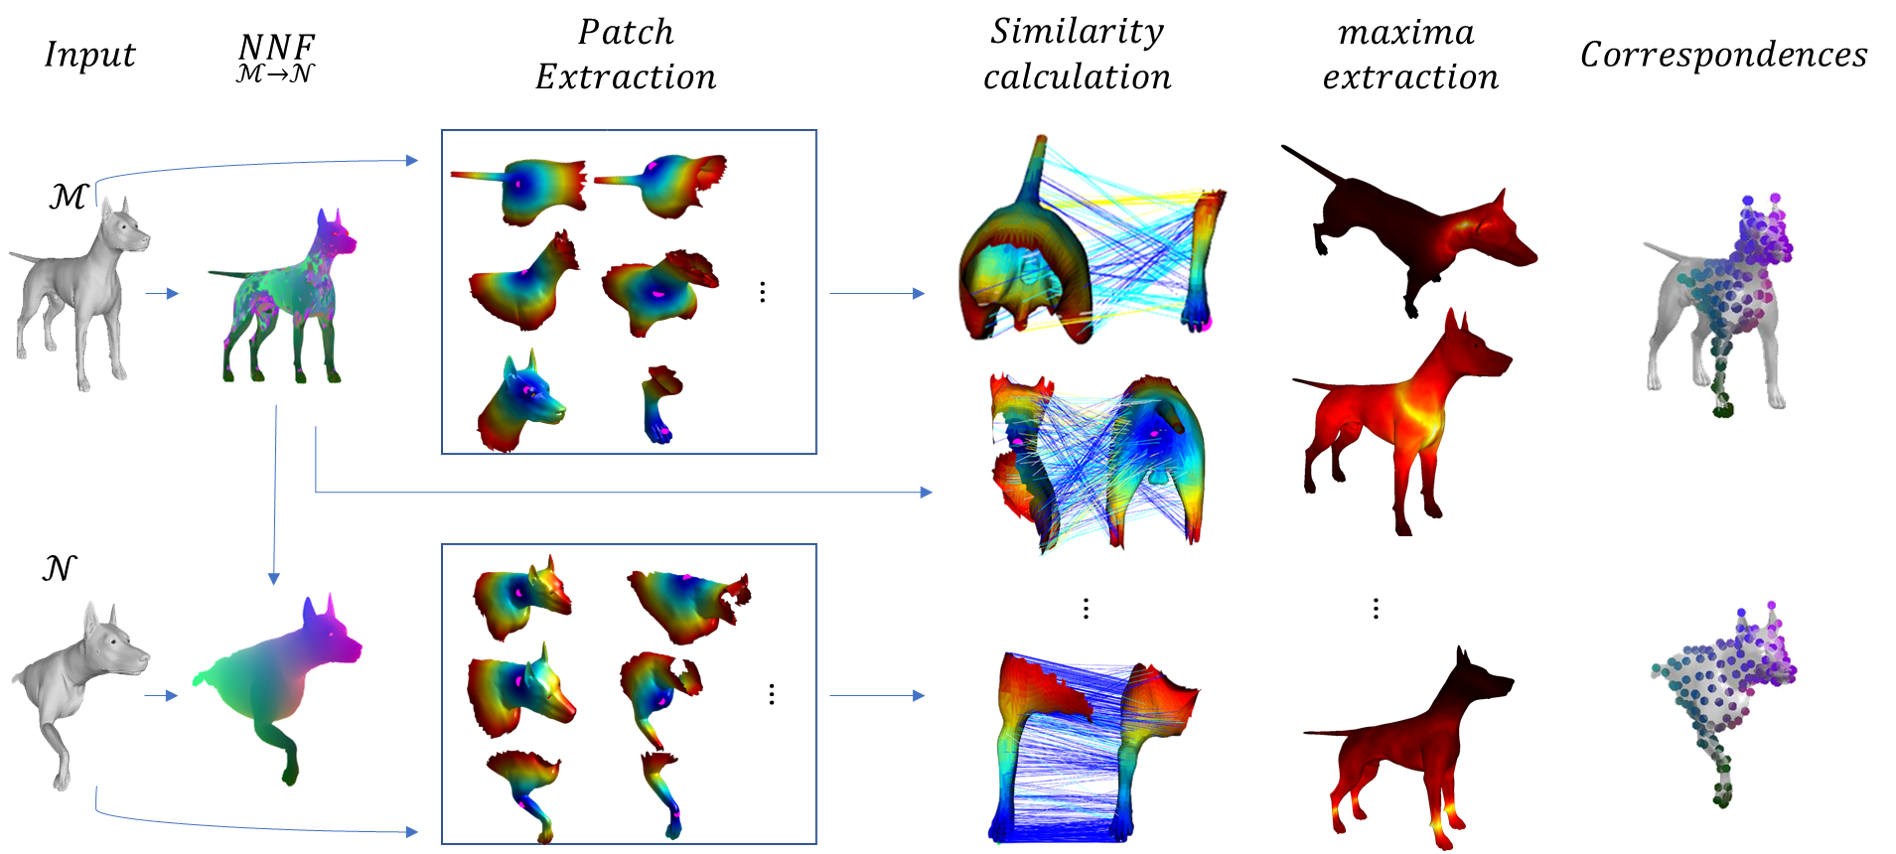
\includegraphics[width=1\textwidth]{figures/Birds_Flight.png}
	\caption{{\bf Algorithm outline.}
    In the first step, we compute the nearest-neighbor field for $\mathcal{N}$ and $\mathcal{N}$.
    Then, patches of the surfaces are extracted for every sample point in $\mathcal{N}$ and for every vertex on $\mathcal{M}$.
    These patches cover the surface (i.e., may overlap) and represent semantic regions. 
    Note that exact segmentation is not needed.
    Step 3 is the core of the algorithm, in which the similarity between the patches is computed.
    Finally, in Step 4, for every sample of $\mathcal{N}$ we set the vertex of $\mathcal{M}$ that achieves the maximal score as its corresponding point.
	\ayellet{This figure should be re-done} 
	}
	\label{fig:overview}
\end{figure*}

Given two surfaces $\mathcal{M}$ and $\mathcal{N}$, the goal is to find the best match of  $\mathcal{N}$ within  $\mathcal{M}$.
In particular, we aim at extracting a sparse set of point correspondences between the models. 
Our approach is based on three key ideas, which we describe hereafter.

%%%%%%%%%%%%%%%%%%%%Key Idea underlying the original DDIS : diversity
First, inspired by \cite{talmi2017template}, similarity is captured by two properties of the Nearest Neighbor field. 
(1) When $\mathcal{N}$ and a patch of $\mathcal{M}$ match, most points in $\mathcal{M}$ have a unique NN-match in $\mathcal{N}$. 
This implies that the NN field should be highly diverse, in the sense that many different points in $\mathcal{N}$are being matched.
(2) Arbitrary matches typically imply a large deformation, whereas correct matches should preserve the distance between pair of points.
Therefore, Similarity should be based both on the diversity of the Nearest-Neighbor field and on the consistency of the distances between the points.

% One key to our method is the assumption that while non rigid deformations and partiality leads to changes in the data, the underlying shape distributions from which the shapes on the surfaces are drawn should remain highly overlapping, and thus the data points drawn from these should be spread approximately uniformly, one inside the other, leading to a high diversity of nearest neighbors.
% %%%%%%%%%%%%%%%%%%%%%The idea underlying our improvement%%%%%%%%%%%%%%%%%%%%%%%%%%%%
% However, since unlike in\cite{talmi2017template} we don't have the benefit of having a template and a query of the same size in the absence of a grid, and the space of geometric shapes is more constrained then that of RGBXY, one should not expect a near bijection. 
%%%%%%%%%%%%%%%%%%%%Key Idea underlying the original DDIS : low deformation%%%%%%%%%
% Another assumption is that of a geometrical coherency  - geodesic distances of corresponding pairs of points on a shape and a roughly isometrically deformed version of which should hold approximately leading us to use the assumption of low distortion.
%%%%%%%%%%%%%%%%%%%%%%%%%%%%%Our added observation%%%%%%%%%%%%%%%%%%%%%%%%%%%%%%%%%
% However, the preservation of distances holds only approximately even for full template matching, and even less so in the presence of partiality and topological noise.
% It holds that the longer a distance between 2 points is, the more likely it is that a distortion had occurred on the geodesic path between them, either due to a non isometric deformation, partiality removing a piece of the geodesic path or topological noise introducing a shortcut.
% It follows from this that the smaller the pieces we are trying to match will be, the higher the likelihood of pairwise distances to be preserved should be.
Second, rather the realizing the similarity test, described above, on $\mathcal{N}$ as a whole, it is preferable to perform it on a set of small sub-surfaces of $\mathcal{N}$.
This is so not only since a small sub-surfaces is more likely to exhibit consistent distances, but also since it is less likely to be matched to a repeating pattern, which would lead to smaller diversity.

Third, a multi-scale approach with respect to the size of matched sub-surfaces is beneficial.
This is so since larger surfaces contain more global context, resulting in matches which lie in a correct region, but provide poor localization. 
On the other hand, matching smaller surfaces lead to results which are better locally, but may be globally inconsistent. \ayellet {what do you mean by globally inconsistent?}

Therefore, our algorithm, which is illustrated in Figure~\ref{fig:overview}, consists of the following steps.
\begin{enumerate}
    %%%%%%%%%%%%% Step 1
    \item 
    \textbf{Pre-processing}.
    Shape descriptors are calculated for every vertex of both meshes and an approximate nearest neighbor field is computed for the vertices, as described hereafter.
    
    Many descriptors have been proposed in the literature~\cite{rusu2008towards,tombari2010unique,Sun:2009:CPI:1735603.1735621}.
    We use the FPFH~\cite{rusu2009fast}, which is robust to small deformations and partiality of the data, yet sensitive to symmetrical flips.
    \ayellet{what makes it sensitive to symmetrical flips?}
    Therefore, it addresses a major drawback of matching a right arm, for example, to the left one.
    %
    We then compute a nearest neighbor field mapping, by assigning each vertex of $\mathcal{M}$ its nearest neighbor in $\mathcal{N}$, FPFH-wise.

    %%%%%%%%%%%%% Step 2
    \item
    {\bf Patch extraction.} 
    Inline with the second key idea, we aim at extracting a meaningful set of sub-surfaces, which cover (rather than partition) the surface.
    This is done in two steps:
    First, we extract a meaningful set of points, whose neighborhoods provide a good cover of the surface. 
    We then extract the patches using this sample.
    We elaborate hereafter.
    
    To extract the sample point set, we start from the extremities of the surface, which are considered salient points.
    A vertex is considered to be an extremity if it  resides on a tip of the surface (e.g.,  tips of limbs)~\cite{katz2005mesh},
    In practice, we define them to be vertices that are local maxima of the sum of the geodesic distance functional.
    Formally, $\forall v \in S$,  let $N_v$ be the set of neighboring vertices of vertex $v$. 
    Let $GeoDist(v_i, v_j)$ be the geodesic distance between vertices $v_i$ and $v_j$ of mesh S. Vertex $v$ is an extremity if it satisfies
     \begin{equation}
        \sum_{v_i\in S} GeoDist(v,v_i)>\sum_{v_n\in S} GeoDist(v_n, v_i).
        \label{eq:extremities}
    \end{equation}

    Then, we iteratively add more samples, choosing the next sample point as follows.
    We construct a "forbidden" region around every point in the set.
    This region is a geodesic disc of radius $ 0.05\sqrt{Area(\mathcal{M})}$.
    The next point to be added to the set is a vertex whose geodesic distance to any sample point in the set is minimal and does not fall in any of the forbidden regions.
    This process stops when the entire surface is marked forbidden. 
    % The resulting set of samples is denoted as  $\S_{\mathcal{N}}\in\mathcal{N}$.

    Once the set of representing sample set is defined, a disc (sub-surface) of geodesic distance $R_T$ is extracted around each sample point, which is the sought-after set of patches.
    Specifically, $R_T=\beta\cdot \sqrt{Area(\mathcal{M})}$.
    As our approach is multiscale, $\beta$, which was found empirically by minimizing the error of correspondences on a training set, varies. 
    In practice we use $\beta=\{0.6,0.4,0.2\}$.
 
 %   \nadav{We repeat this process for every $m\in\mathcal{M}$ to create a set of geodesic discs $\{{\mathcal{M}_{m_j}^{R_T}}\}_{j=1}^{|\mathcal{M}|}$}
    
    %%%%%%%%%%%%% Step 3
    \item
    {\bf Computing similarities between pairs of patches.} 
    This step is the core of our algorithm, which realizes the first key idea.
 
    For each pair of patches of the same scale, $Q_i \subset \mathcal{M}$ and $P_i \subset \mathcal{N}$, we compute a similarity value.
    %
    Recall that our goal is to reward a nearest-neighbor field with high diversity and low deformation. 
    We will define the similarity function $DDIS$ that achieves it  in Section~\ref{sec:similarity}.
    This is done in a multi-scale manner.

    % \textbf{Refinement.} The goal of this stage is to achieve better correspondences based on simple global tests and constraints
    % \begin{itemize}
    % \item Correspondences which exhibit high distortion are determined are marked as not trusted.
    % \item For Correspondences which are deemed not trusted we search among the local maximas of the DDIS score a point which minimizes their distortion w.r.t to trusted point.
    % \end{itemize}
    
     %%%%%%%%%%%%% Step 4
   \item{\bf Extracting a sparse set of corresponding points.}
    Given the similarity values between the patches, our goal now is to extract a set of corresponding points between  $\mathcal{N}$ to $\mathcal{M}$.
    If we had a single scale, then for each sample point (the center of a patch) of $\mathcal{N}$, we would choose the vertex of $\mathcal{M}$ that maximizes the similarity function.

    In our multi-scale approach, we proceed from coarse to fine.
    Suppose that $P_i \subset \mathcal{N}$ and $Q_j\subset \mathcal{M}$ were found to have the highest similarity in a coarsest scale (i.e. $Q_j$ is the largest).
    The coarsest match is then set between $v_i \in P_i$ and $w_j \in Q_j$, where $v_i, w_j$ are the {\em geodesic centers} of  $P_i, Q_j$, respectively (i.e. the sample points that define the patches in Step 2).
    When moving to the finer scale, we replace  $Q_j$ with a smaller (finer) patch in which $w_j$ is the center and set the new $w_j$ to be the vertex on this patch that  maximizes the similarity function $DDIS$ on this patch.
    The finest $w_j$ is the corresponding point of $v_i$; see Figure~\ref{fig:multiscale}.
    
    \begin{figure}[htb]
	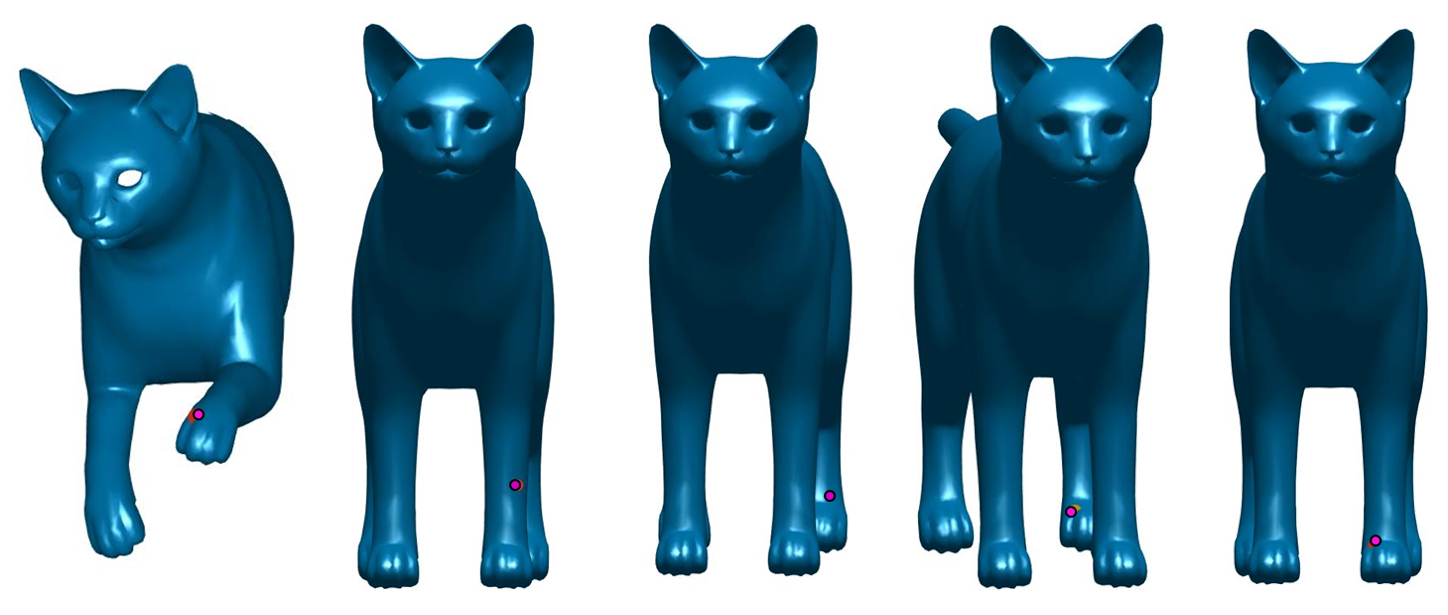
\includegraphics[width=0.5\textwidth]{figures/MultiScaleDis.png}
	\caption{{\bf Multi-scale similarity.} 
	Given the sample point on the left (in magenta), the corresponding points on  $\mathcal{M}$ are shown on the right. 
	In the coarsest level, the general region of the matching point is found, but the point is imprecise.
	In subsequent levels, the general region is not found.
	Our multi-scale approach manages to find the precise point.
	\ayellet{Replace the image.} \nadav{done}
	}
	\label{fig:multiscale}

    \end{figure}

    \item{\bf Coherency-based correspondence refinement}
    The result of Step 4 is a set of corresponding pairs of points.
    In most cases ($>92\%$ on all our examples), the correspondences are correct.
    The goal of this step is to identify the incorrect ones and replace them by the correct correspondences. 
    
    The key idea is to utilize coherency, i.e., if all points in the neighborhood of point $v \in \mathcal{N}$ are mapped to points that reside on the same region on $\mathcal{M}$,  it is expected that the corresponding point of $v$,  $w \in \mathcal{M}$, will also reside in this region.
    In other words, we are looking for outliers of the mapping.
    
    To detect these outliers, we check the sum of geodesic distances. 
    For a pair of points $(v,w)$ to be considered correct, they should satisfy:
    \begin{equation}
    \label{eq:refinement}
        \sum_{v_i\in \mathcal{M}}|{GeoDist(v,v_i)} - {GeoDist(w,w_i)}| < C
    \end{equation}
    where $w_i$ is the corresponding point of $v_i$ and $C$ is $0.15$ of the mean of Equation~\eqref{eq:refinement} on all points.
    We replace the corresponding point of an outlier by a point that minimizes Equation~\eqref{eq:refinement} and is a local maximum of the similarity function of Step 3.

\end{enumerate}

% \nadav{proposed end of section}
% \nadav{comment: This should not be in the final version .
% I had embedded this into the Similarity calculation and sparse correspondences section. hopefully it makes more sense there}
% The latter \ayellet{two steps} are performed in a multi-scale approach. 
% To do it, we define a set of $N$ scales, which define geodesic radii $R_{T_1}>...>R_{T_N}$, \ayellet{which are the pre-defined thresholds of Step 2}\nadav{No, they are not. The density of sampling radius used for step 2 is not the same as the radius we use to construct our geodesic discs}.
% The larger the radius, \ayellet{the ....}
% \ayellet{ I do not understand anything you say below. Do you use the results in one scale to calculate the other. How is Step 3 influenced?}\nadav{At step 3 we calculate k similarity scores for each pair of points - one for each geodesic disc radius $R_{T_k}$}
% \nadav{We then move from a coarse to fine scale by iteratively finding the maxima of similarity at scale $R_{T_k}$, and use to define a valid set of points from which we pick the maxima at scale $R_{T{k+1}}$ by constraining them to lie in a geodesic disc of radius $R_{T_k}$ around it. We repeat this process and determine the final correspondence at scale $N$}

%%%%%%%%%%%%%%%%%%%%%%%%%%%%%%%%%%%%%%%%%%%%%%%%%%%%%%%%%
%%%%%%%%% section: Similarity
%%%%%%%%%%%%%%%%%%%%%%%%%%%%%%%%%%%%%%%%%%%%%%%%%%%%%%%%%
\section{Similarity}
\label{sec:similarity}
\begin{figure}[htb]
	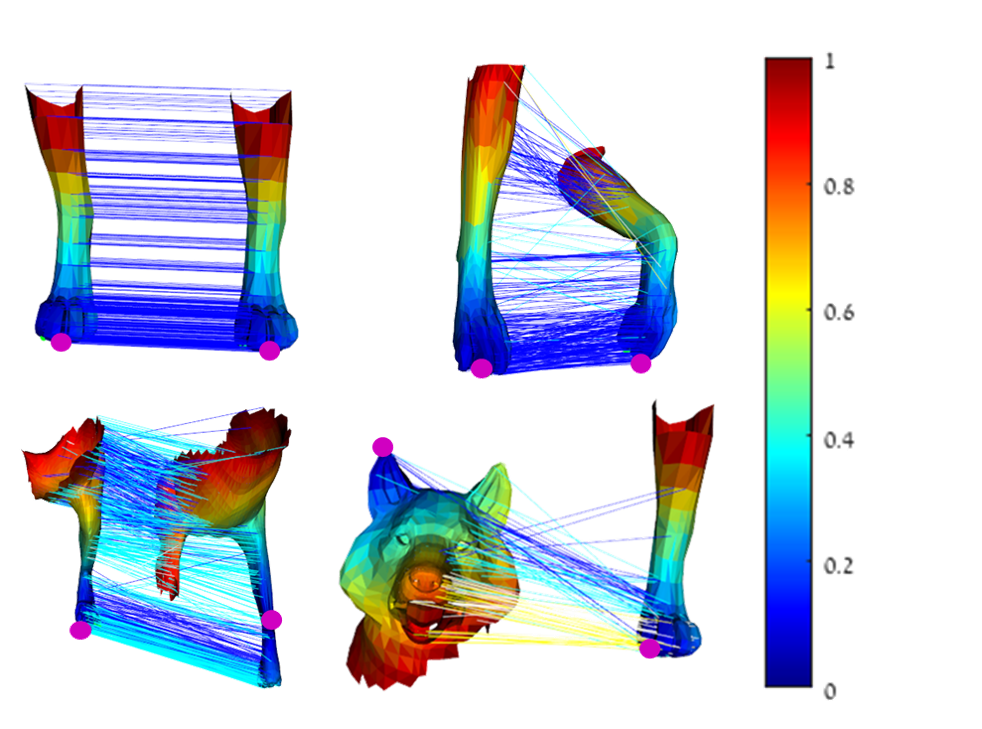
\includegraphics[width=0.5\textwidth]{figures/DDIS2.png}
	\caption{{\bf Nearest Neighbor Field.} 
		The surfaces are colored by the geodesic distances from the magenta point; the lines are colored by the \nadav{difference of geodesic distances from the purple point}. \ayellet{deviation of what?} 
		Clearly, similar surfaces on the top (even when deformed) exhibit diversity in matching (i.e. different points on one surface are matched to different points on the other).
		Furthermore, in this case, most lines are blue, which indicates similar distances from the source point.
		This is not the case at he bottom, where the surfaces are highly different from one another.
		}
		\label{fig:NNF}
\end{figure}

%Problem definition
This section elaborates on Step 3, which is the core of the algorithm.
Given pair of patches of the same scale, $Q \subset \mathcal{M}$ and $P \subset \mathcal{N}$, this section defines a similarity function, termed {\em 3D Deformable Diversity Similarity (3D-DDIS)}, between them.
This function should be oblivious to non-rigid transformation, different resolutions of the meshes, noise, and partiality of the data.

%Key idea
Recall that the key idea is to reward a point (center of the patch) whose nearest-neighbor field satisfied two properties: it has both high diversity and low deformation. 
As for diversity, when $Q$ and $P$ correspond, most of the points on $Q$ points have a unique NN-match on $P$. 
Conversely, if $Q$ and $P$ do not correspond, most of the points on $Q$  do not have a good match on $P$, and therefore the nearest neighbors are likely to belong to a small set of points that happen to be somewhat similar to the points of $Q$.
This implies that the NN-field is highly \textit{diverse}, pointing to many different points in $P$.
In addition, if two patches correspond, pairs matching (nearest neighbors) points tend to have similar geodesic distances to the centers of the patches they reside on.
Conversely, arbitrary matches typically do not maintain such distances.
\ayellet{why is it called deformation?}

To realize these requirements, we start by formally defining the diversity, $Div(Q,P)$, and  the deformation, $Def(Q,P)$, and then show how to put them together into a similarity function.
An intuitive and efficient way to measure diversity is to count the number of unique NNs between the points of  $Q$ and $P$:
\begin{equation}
\label{eq:diversity}
Div(Q,P)=|\{p_i\in P:\exists q_j\in Q,NN(q_j,P)=p_i\}|,
\end{equation}
where  $\{p_i\}_{i=1}^{|P|}$ and $\{q_j\}_{j=1}^{|Q|}$ are the set of points of $Q$ and $P$, respectively and the nearest neighbors is computed between the descriptors (FPFH) of the points.
However, we will see below that the diversity can be calculated implicitly.

Next, we define $Def(Q,P)$, the deformation from  $Q$ to $P$.
Let $p \in P$ and $q \in Q$ be the centers of $P$ and $Q$, respectively;
furthermore, let $p_i= NN(q_j,P)$ be the nearest-neighbor of  $q_j \in Q$.
The deformation implied by the NN-Field for ${p_i,q_j}$ is defined by:
\begin{equation}
def(q_j,p_i,Q,P)= |{GeodDist(q_j,q)-GeodDist(p_i,p)}\epsilon|,
\end{equation}
where $0<\epsilon << Area(\mathcal{M})$ and is a used for numerical stability.

For each $p_i \in P$, we find the minimal deformation $r_i^*=min_{q_j \in Q}def(q_j,p_i,Q,P)$ such that $p_i$ is the nearest neighbor of $q_j$.
Note that some points in $P$ might not be associated with any point in $Q$ (since they are not the nearest neighbors of any point $q_j\in Q$);
in this case $r_i^*=\infty$.

Having defined diversity between patches and deformation between points on these patches, we define the similarity between patches $p$ and $Q$ as:
\begin{equation}
DDIS(P,Q)=\sum_{p_i\in \mathcal{P}}\frac{1}{1+r_i^*}.
\label{eq:DDIS}
\end{equation}

It is easy to see how the 3D-DDIS rewards low deformation.
However, we will explain hereafter why it also rewards high diversity.
Consider a case where $r_i^*\in\{0,\infty\} \forall p_i$. 
When this occurs $\frac{1}{(1+r_i^*)}\in\{1,0\}$ and it indicates that a point $p_i$ has a point in $Q$ that considers $p_i$ to be its nearest neighbor.
In this scenario, 3D-DDIS simply counts the number of points in $Q$ that are nearest neighbors of some point in $P$.
But, this is precisely the diversity function we seek-after.
\ayellet{copy a convincing explanation for the general case}
\nadav{
In the general case, the contribution of every point is inversely weighted by its deformation $r_i^*$, which gives preference to plausible deformations of real objects.
}

%% In the thesis, in the results section add a paragraph where you explain this image
% \begin{figure}[htb]
% 	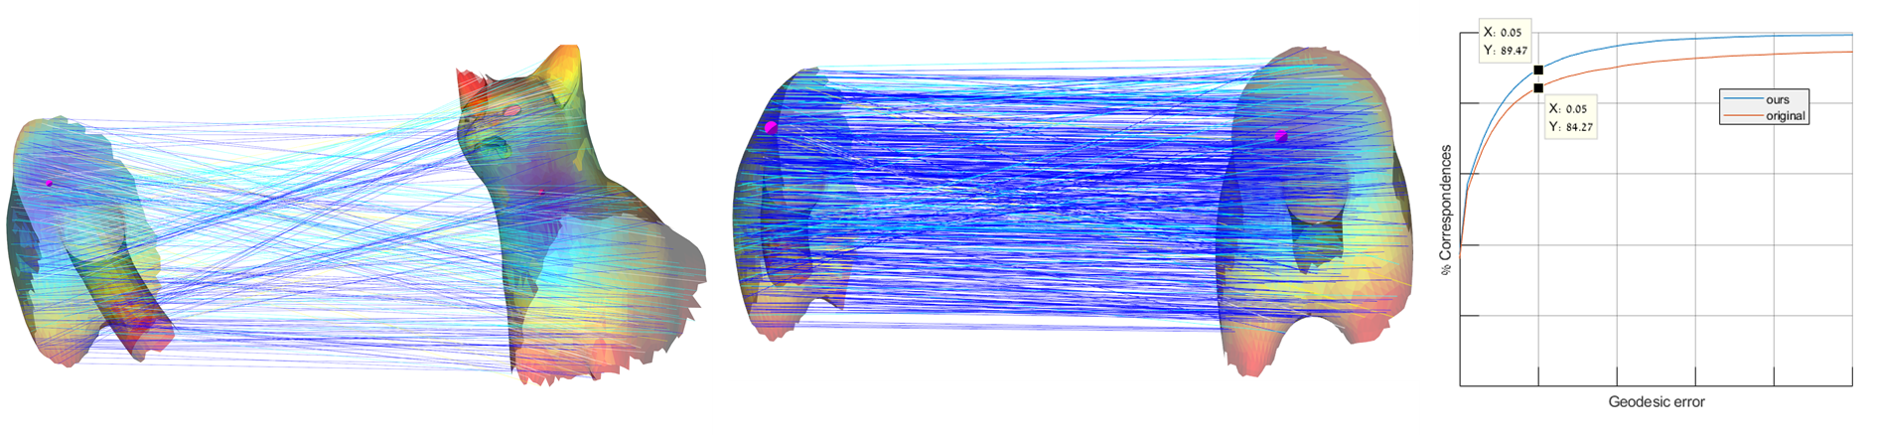
\includegraphics[width=0.5\textwidth]{figures/DDISvsWDIS.png}
% 	\caption{Qualitative and quantitative illustration of the improvement introduces by our formulation. On the top left the Nearest neighbor mapping between the part and its corresponding ground truth geodesic disc. As can be seen low distortion is occurring between the true corresponding points, but the symmetrical part which is not included on the partial model maps to the same points - thus attenuating the score originating from these. One the bottom left we see the piece chosen by the original DDIS formulation. The arrows with low distortion seldom have other points which are their nearest neighbors and thus achieves a better score without our modification. The cumulative error curves show an improvement of ~5 percent on the training set using our formulation.}
% \end{figure}

%%%%%%%%%%%%%%%%%%%%%%%%%%%%%%%
%%%%%%% Section: Results
%%%%%%%%%%%%%%%%%%%%%%%%%%%%%%%
\section{Results}
\label{section:results}
\begin{figure*}[htb]
	\label{Shrec16Qualitative}
	\centering
	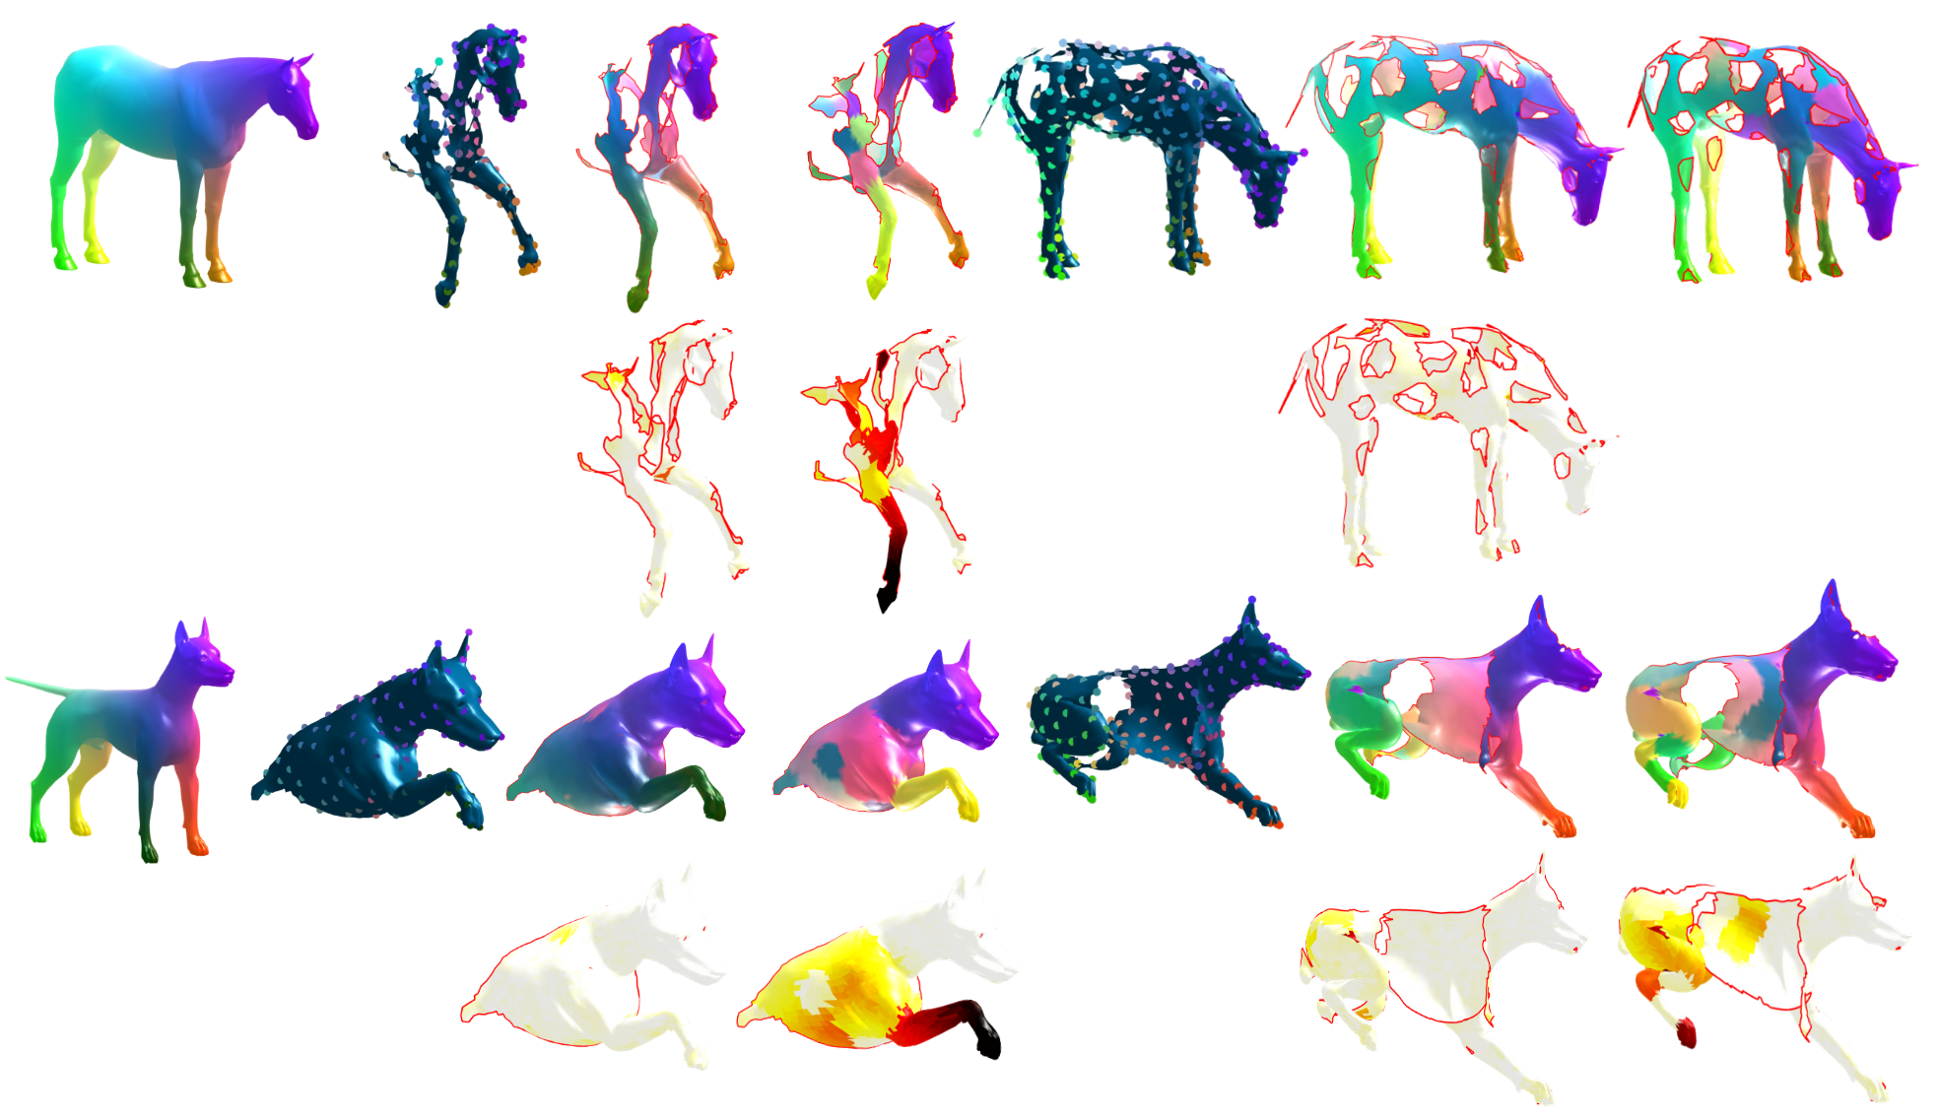
\includegraphics[width=1\textwidth]{figures/SHREC16Partial.png}
	\caption{Results on Shrec'16 partial benchmark. in the right column we have the null shape. Each part triplet includes our sparse result, the dense correspondence extension, and the result obtained by PFM\cite{rodola2017partial}. Below each dense correspondence we illustrate the geodesic error.}
\end{figure*}


\ayellet{first paragraph: generally the datasets we ran on}
\nadav{We have evaluated our method both qualitatively and quantitatively on the challenging benchmarks of SHREC 16 Partial Matching of Deformable Shapes\cite{cosmo2016shrec}and SHREC’16: Matching of deformable shapes with topological noise\cite{lahner2016shrec}, achieving results comparable or better to state of the art on both.}
\paragraph{Qualitative results:} xxx

\ayellet{second paragraph: qualitative results - images + comparisons + explanation}
\nadav{We provide a qualitative visual evaluation of our method along with a comparison to the method with that of \cite{rodola2017partial} in the case of the Partial Matching of Deformable Shapes dataset in Fig~\ref{Shrec16Qualitative} and on the Topological Noise dataset in Fig~\ref{Shrec16TopImage}. 
It can be seen  that our method can obtain sparse correspondences of a high quality, which can be then turned into dense ones with negligent loss of quality by feeding them to the method of \cite{litany2017fully} as delta functions. 
Our methods explicit usage of distance preservation tends to result in more coherent solutions and mostly avoid symmetrical assignments, which plague \cite{rodola2017partial}. 
The improvement is especially felt in the case of the holes dataset.
On the topological noise benchmark we can see bad matches are typically limited to the area of the topological noise, while PFM breaks completely on occassions.}

\paragraph{Quantitative results:} xxx
\begin{figure}[htb]
	\label{Shrec16Cumulative}
	\centering
	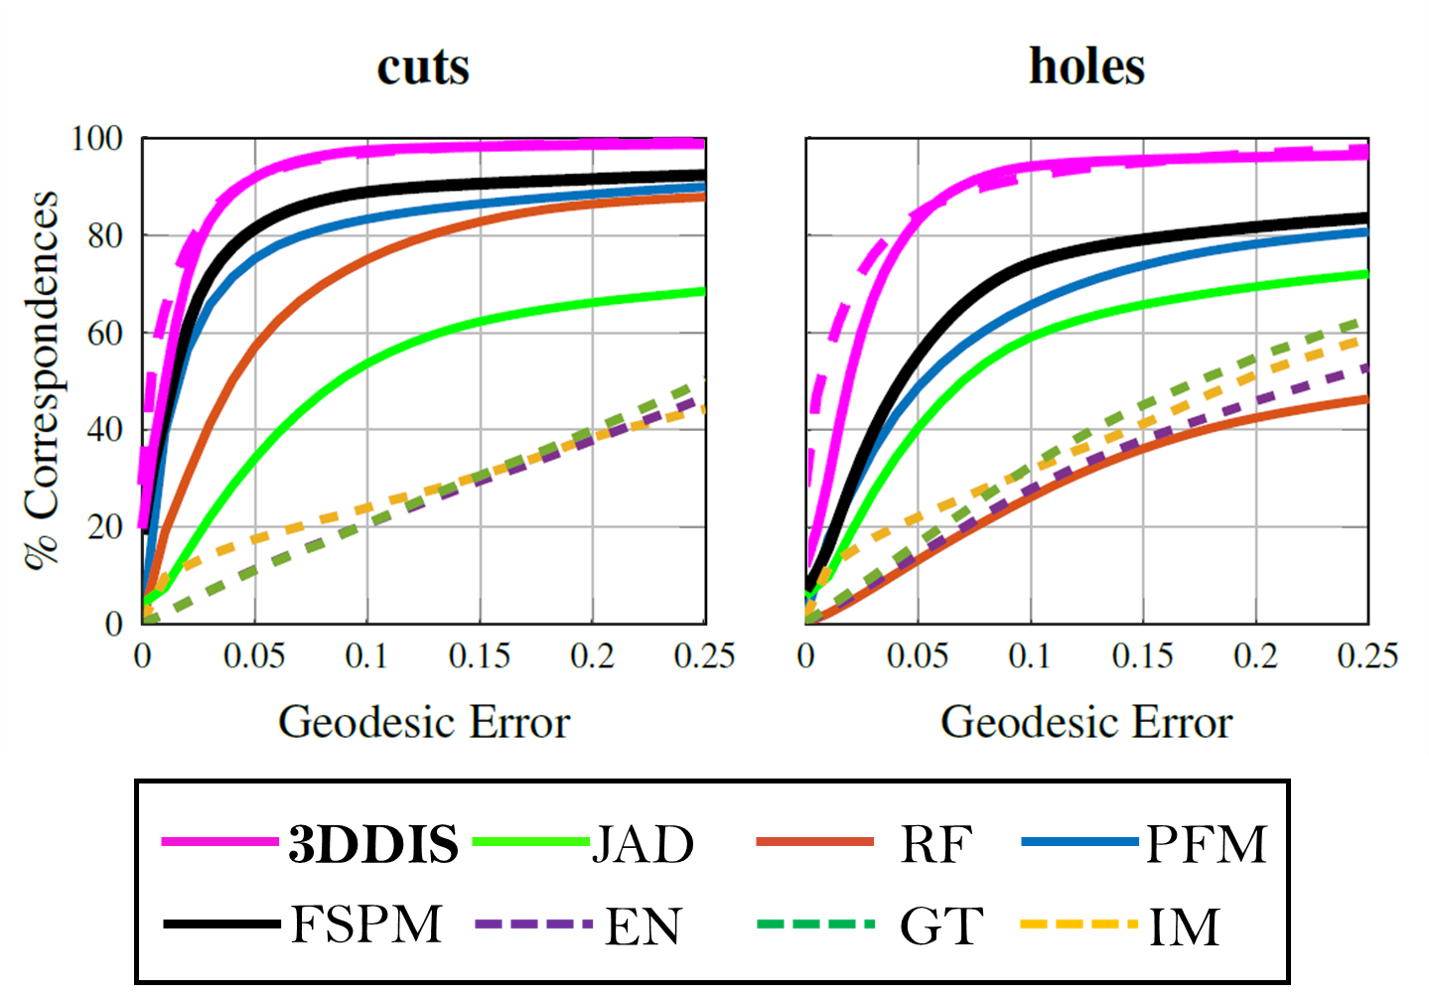
\includegraphics[width=0.5\textwidth]{figures/ROCSHRECCumulative16.png}
	\caption{Cumulative geodesic error curves on Shrec16 Partial matching benchmark. Our method is illustrated in magenta}
\end{figure}
\begin{figure}[htb]
	\label{Shrec16Part}
	\centering
	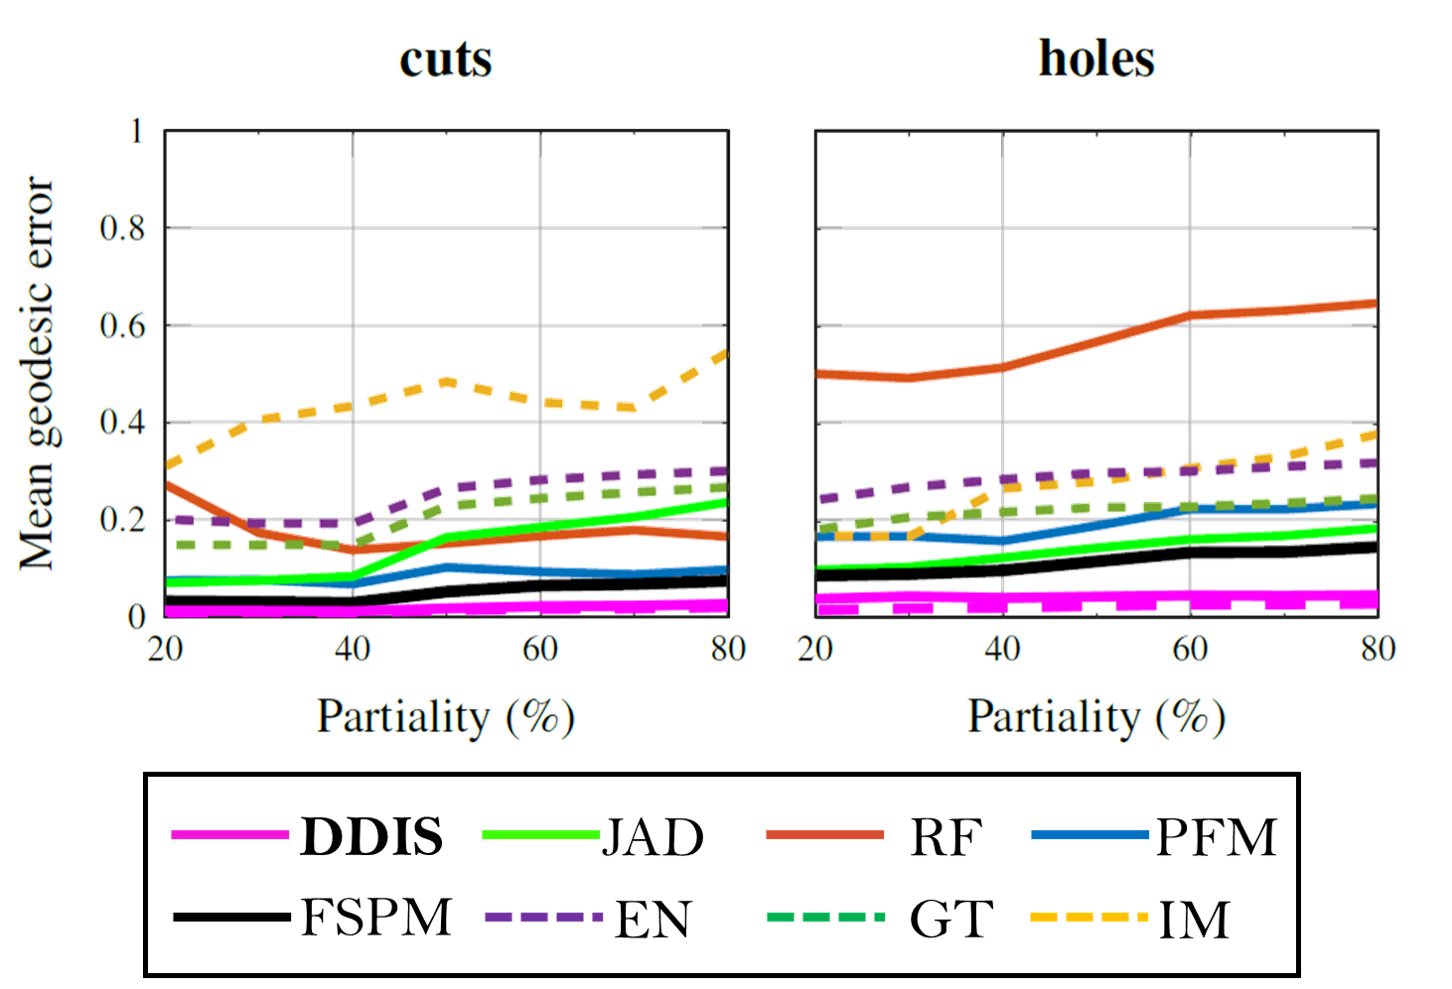
\includegraphics[width=0.5\textwidth]{figures/ROCSHREC16Part.png}
	\caption{Error as a function of model partiality.}
\end{figure}
\ayellet{next paragraphs: quantitative results - explain the datasets in one paragraph, the error metrics in one paragraph, and explanations of the graphs+tables/results - one paragraph per graph}
\nadav{We provide quantitative evaluation of our method on both datasets w.r.t previously reported results on the benchmarks.
\subparagraph{Error Metrics}
We evaluate correspondence quality according to the princeton benchmark protocol\cite{kim2011blended} detailed hereafter. 
Given a correspondence points $(q,p)\in \mathcal{N}\times \mathcal{M}$ produced by an algorithm, when the ground truth correspondence is $(q,p*)$. The error of the said correspondence is measured by the normalized geodesic distance on $\mathcal{M}$:
\begin{equation}
\varepsilon(q)=\frac{GeoDist_{\mathcal{M}}(q,p^*)}{\sqrt{area(\mathcal{M})}}
\end{equation}
We plot cumulative curves showing the percentage of errors falling below a variable threshold. 
Symmetric solutions are accepted with no penalty.
We report results both for the sparse correspondences produced by our algorithm, and dense ones, produced by feeding the former to the method of \cite{litany2017fully}.
\paragraph{Part to Full}
We have carried out a quantitative evaluation of the partial matching scenario on the SHREC'16 Partial Deformable Shapes benchmark. The benchmark contains 400 partial shapes, each a near isometrically deformed version of one of 8 base class.
Each class is provided with a "null" shape in a neutral pose. The partial shapes are further divided into 2 subsets, determined by the type of partiality. 
\textit{cuts}, which is composed of shapes produced by dividing shapes by a plane, and \textit{holes}, obtained by eroding many areas around random vertices. The size of the parts ranges from ~800-9k vertices.
We report our results in Figures ~\ref{Shrec16Cumulative}\ref{Shrec16Part}. We compare them with the results reported in Fully Spectral Partial Matching(FSPM)\cite{litany2017fully}, which also compares results with partial functional maps(PFM)\cite{rodola2017partial}, random forests(RF), scale-invariant isometric matching(IM), game-theoretic matching(GT), elastic net matching(EN) and joint diagnolization. 
Methods producing sparse matches are marked in a dashed line, whereas full correspondences are marked with a full line. 
We produced the graphs for our method using the code provided in the benchmark site.
We can see from the plots that our method produces a considerable improvement over the previous state of the art method of FSPM. 
On the cuts dataset an improvement of ~10\% is seen while an impressive 20\% is achieved over the holes dataset.

\paragraph{Topological changes}
\begin{figure}[htb]
	\label{Shrec16Top}
	\centering
	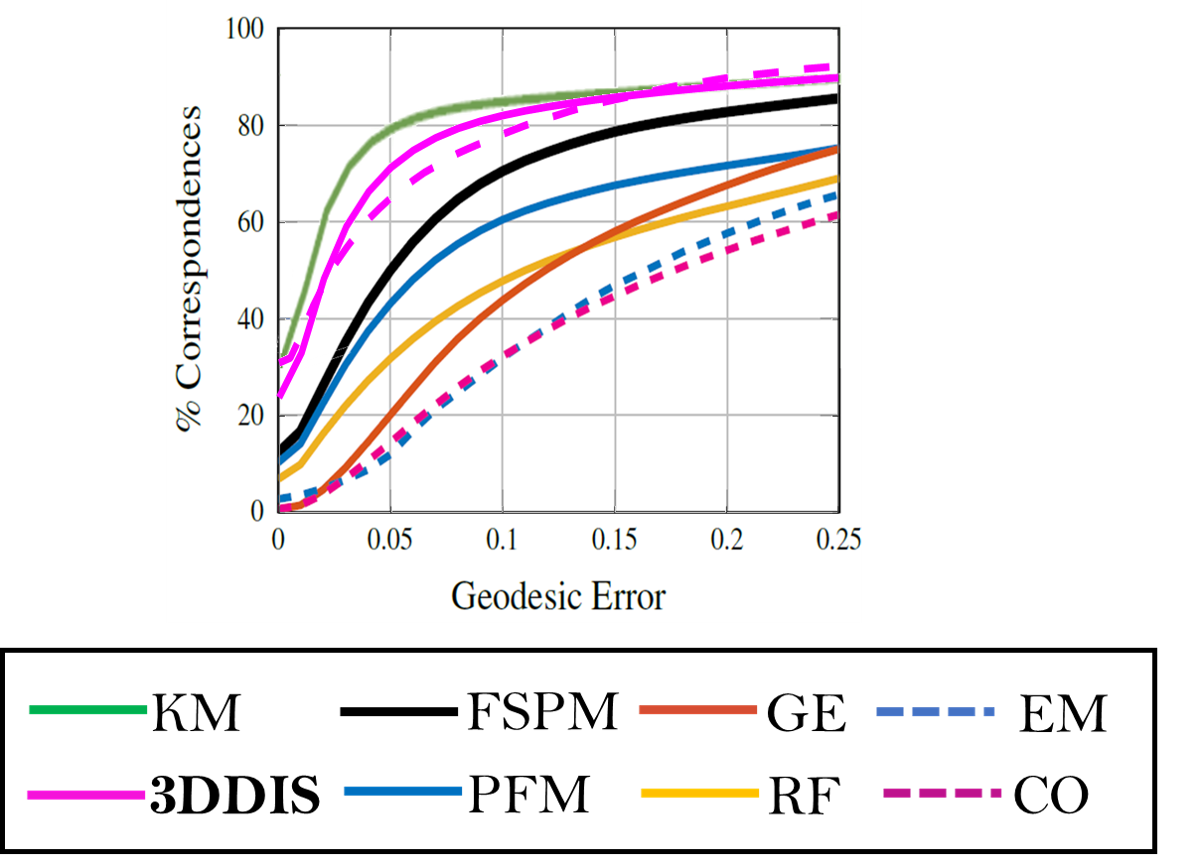
\includegraphics[width=0.5\textwidth]{figures/SHREC16Top.png}
	\caption{Cumulative error curve on SHREC 16 Topology benchmark.}
\end{figure}
\begin{figure}[htb]
	\label{Shrec16TopImage}
	\centering
	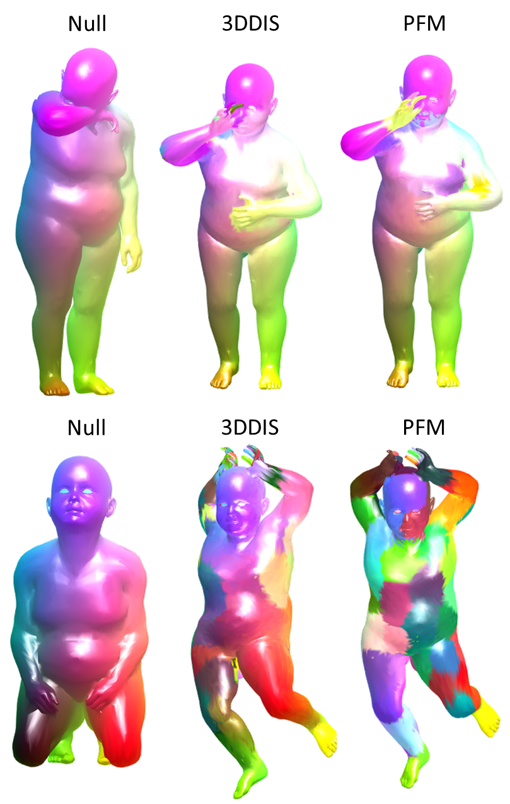
\includegraphics[width=0.5\textwidth]{figures/SHRECTopology.png}
	\caption{Improvements achieved by our method on the SHREC Topological Noise benchmark.}
\end{figure}

We have also performed a quantitative evaluation on the SHREC 16 Topological noise benchmark\cite{lahner2016shrec}. The low resolution benchmark includes 10 shapes with ~10K vertices each, derived from the same base human shape which undergoes deformations and topolgical changes stemming from self intersection. Each shape is matched to all the others resulting in 90 matching problems. We compare our results with those reported in\cite{vestner2017efficient} in Figure ~\ref{Shrec16Top}.

We can see from the plot that we fall short of achieving state of the art results on this benchmark. The additional paths between points introduced by topological noise causes significant problems in matching, especially around the noisy areas, a fact that\cite{vestner2017efficient} manages to tackle partially by optimizing over different distance kernels along with descriptor similarity. It might be worthwhile to find a way to incorporate these kernels into the 3D-DDIS framework.}

\paragraph{Drawbacks:} xxx
\ayellet{fifth paragraph: drawbacks with examples}
\nadav{Our method exhibits a few drawbacks. First and foremost is the asymptotic runtime - generating geodesic distances has an asymptotic complexity of $O(n^2 logn)$ and computing 3D-DDIS similarity has an asymptotic runtime of $O(|S|n^2)$, which makes running on meshes with more than 15K vertices prohibitive. The algorithm  also has six parameters which should be tuned. Additionally, surface patches such as the cat's tail, which are low in distinct shapes are hard to match. Finally, the method exhibits real difficulty dealing with topological noise.}

\paragraph{Implementation details:} xxx
\ayellet{sixth paragraph: implementation details, how do we move from sparse to dense}
\nadav{Our code which produces the sparse correspondences is implemented entirely in C++ . For geodesics we have used Fast Marching Geodesics adapted from the code published by Ron Kimmel.
FPFH is calculated using the Point Cloud library\cite{} using a radius of $0.03\sqrt(M)$. Nearest Neighbor field is computed with FLANN\cite{} with $\chi^2$ distance. 
The entire code is parallelized using OpenMP. Since computing similarity for a given patch is totally independent from similarity calculations of all other patches the speedup is nearly linear in the number of threads.
To move from sparse to dense correspondence we employ the method of \cite{litany2017fully}, and replace the SHOT descriptors with localized smooth delta functions, effectively skipping straight to the refinement stage of that algorithm. It is also only necessary to run one iteration instead of 5 when using our correspondences to achieve superior quality of correspondences.}

\paragraph{Alternatives:} xxx
\ayellet{sixth paragraph: alternatives---comparison to Lihi's function, parameter tuning}
\paragraph{Alternatives:} xxx
\ayellet{seventh paragraph: uses in archaeology}

\subsection{Experimental Results}
In this section we will briefly go over the available Datasets
\textbf{SHREC 2016 Partial Correspondence}  
The SHREC partial matching dataset\cite{cosmo2016shrec} consists of 8 base, neutral pose models: cat, centaur, dog, horse, wolf, and 3 humans – 2 males, and 1 female, each containing 10,000 vertices except for the wolf which contains only ~4,500 vertices. Each basic model has corresponding deformed partial shapes obtained either by cutting the shape with a plane or by adding holes on a deformed shape. The set has been divided into train and test sets. The train set is composed of 15 cuts for each base models totaling 120 models,and 10 holed shapes for each model for which ground truth point to polygon correspondences has been provided in barycentric coordinates. The test set is composed of additional 200 cuts and 200 holed shapes. We have tuned our parameters only on the 120 pairs of cuts.

\begin{figure*}[htb]
	\centering

	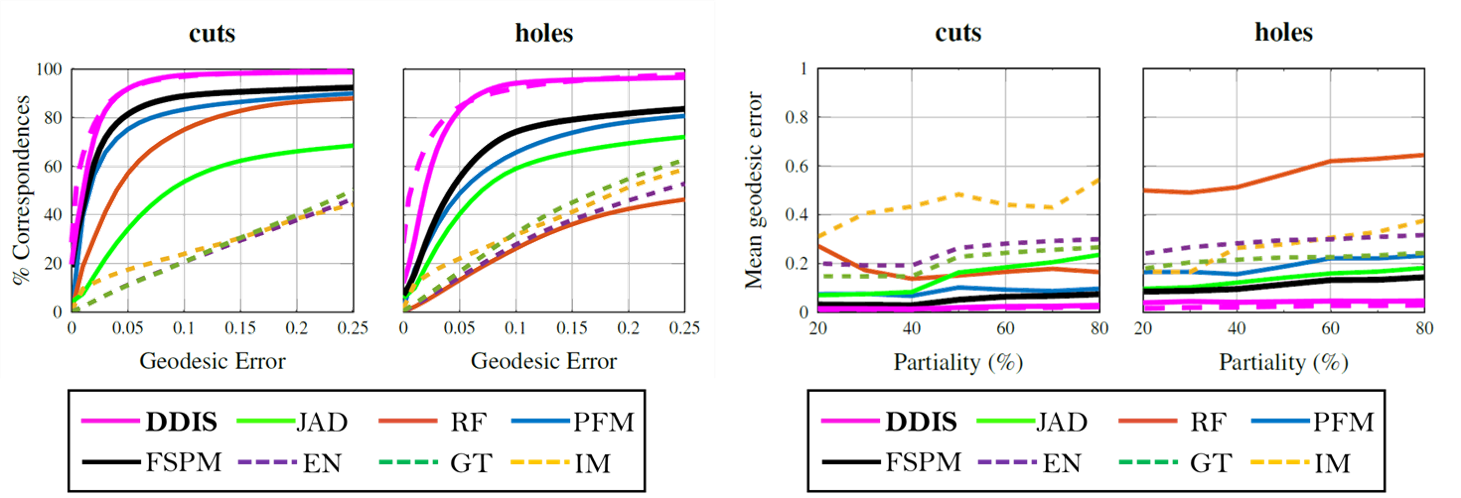
\includegraphics[width=1\textwidth]{figures/ROCSHREC16.png}[htb]
	\caption{comparison with other state of the art algorithms - it can be seen that although sparse in nature, the correspondence obtained by DDIS are much more accurate than the other methods. 
		A separate analysis has been done for correspondences which include boundary points, which tend to be more noisy, and internal points which are more sparse}
\end{figure*}

\subsection{Error Metrics}
The output of partial matching algorithms (as defined in\cite{cosmo2016shrec}) are sub-vertex point-to-point correspondences between partial shapes.
For all experiments we use the standard practice of not penalizing symmetric solutions. Quality is measured according to the Princeton benchmark protocol \cite{kim2011blended}. For a pair of points $(x,y)\in \mathcal{N}\times \mathcal{M}$ between the full object $\mathcal{M}$ and the partial shape $\mathcal{N}$ produced by an algorithm, where $(x,y^*)$ is the ground truth correspondence the inaccuracy is measured by. We plot curves showing the fraction of correspondences whose errors are below a threshold of the normalized geodesic error
\begin{equation}
\varepsilon(x)=\frac{d_{\mathcal{M}}(y,y^*)}{\sqrt{area(\mathcal{M})}}
\end{equation}
where $d_{\mathcal{M}}(y,y^*)$ is the geodesic distance on $\mathcal{M}$, and has units of normalized length on $\mathcal{M}$. For dense correspondences over a dataset, $\varepsilon(x)$ is averaged over all matching instances.

\subsection{Sparse Correspondences on the SHREC16 Test set}
We have tested the performance of DDIS in producing sparse correspondences on the SHREC16 Partial Matching of Deformable Shapes competition. 
We had tuned our parameters on the SHREC16 training dataset using only the cuts part of it. The best results had been produced using FPFH with $r_F = 0.03\sqrt{Area(\mathcal{M}}$, and a piece size radii of $R_T=[0.6,0.4,0.2]\sqrt{Area(\mathcal{M})}$. For Geodesic distances we have found the fast marching algorithm to work the fastest, while giving the lowest error w.r.t. to exact geodesics. For a 10,000 vertices mesh it takes 60s to produce a full distance matrix, Though it should be noted this algorithm has a more efficient GPU implementation, and parallelization on a core brought the run time to ~12s with 6 threads. FPFH and Nearest Neighbor field takes 2s, and similarity between 2 pieces of ~10000 vertices each takes 120s on average, running on 6 threads of i7-4790. Unlike optimization based algorithms this is highly parallelizable.
We achieve results comparable to the state of the art \cite{litany2017fully} quality wise, even though sparser in nature on both the Cuts and the Holes datasets, Where a particularly impressive result is reported on the Holes dataset, which can then be expanded with a minimal loss of quality by feeding these to the FSPM\cite{litany2017fully} as input instead of low level shape descriptors.

\begin{table}[h]
	\centering
	\begin{tabular}{c  c  c  c  c  c  c c} 
		\hline
		& PFM & RF & IM & EN & GT & DDIS  \\ \hline
		cuts & dense & dense & 61.3 & 87.8 & 51.0 & 132.2\\ \hline
		holes & dense & dense & 78.2 & 112.6 & 76.4 & 77.3 \\ \hline
		
	\end{tabular}
	\caption{mean number of correspondence obtained by the algorithms in the SHREC 16 competiton and our algorithm. Note that our algorithm can combine wi}
	\label{table:1}
\end{table}

\begin{figure*}[htb]
	\centering

	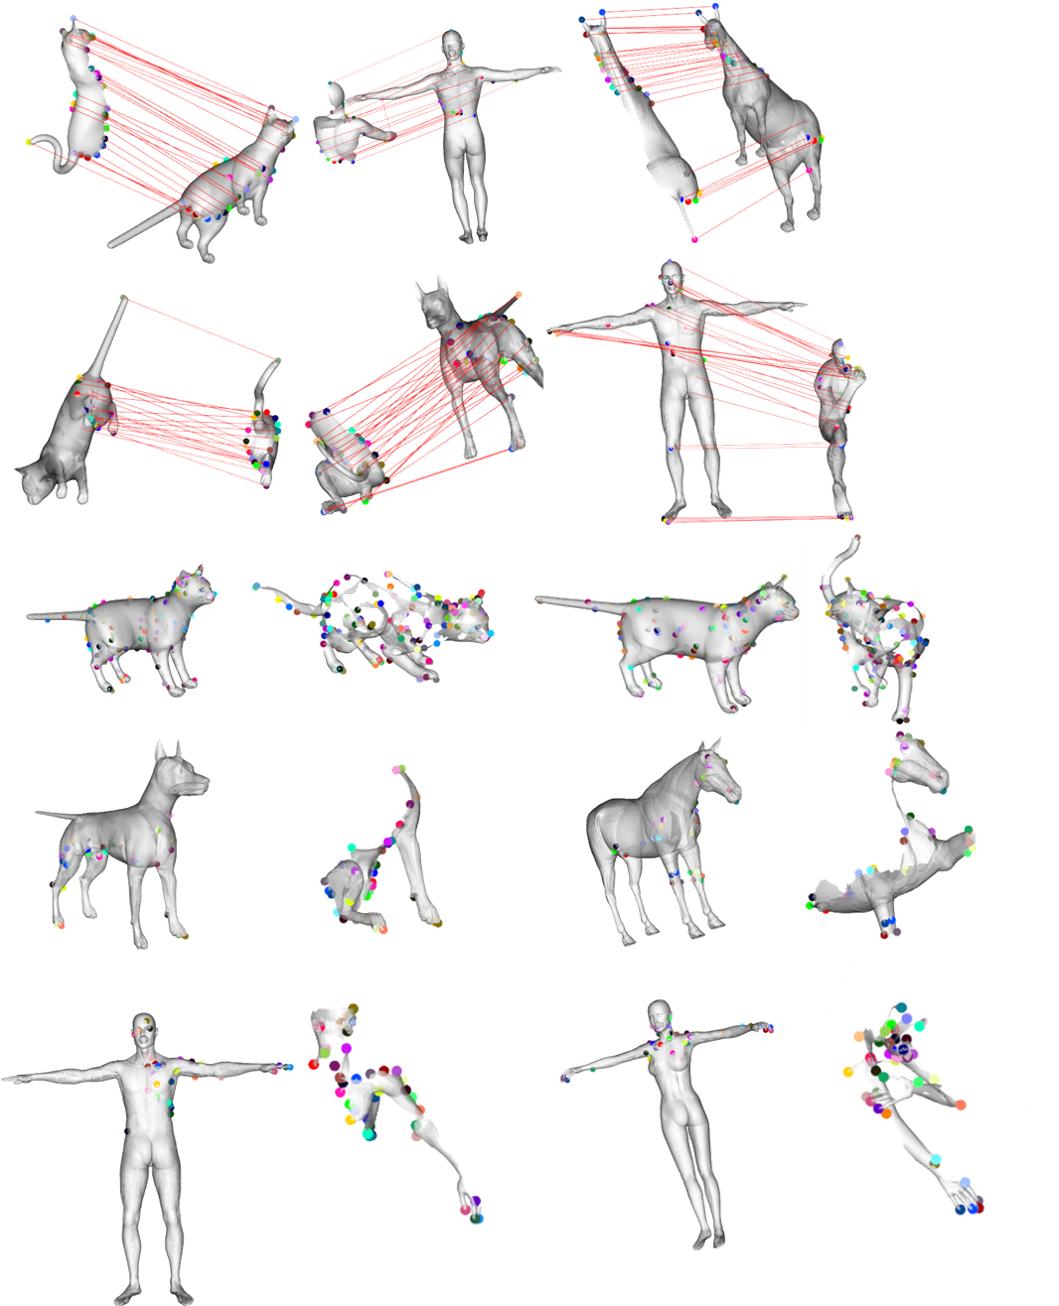
\includegraphics[width=1\textwidth]{figures/success_1}
	\caption{Good correspondences obtained by our method}
\end{figure*}


\begin{figure*}[htb]
	\centering
	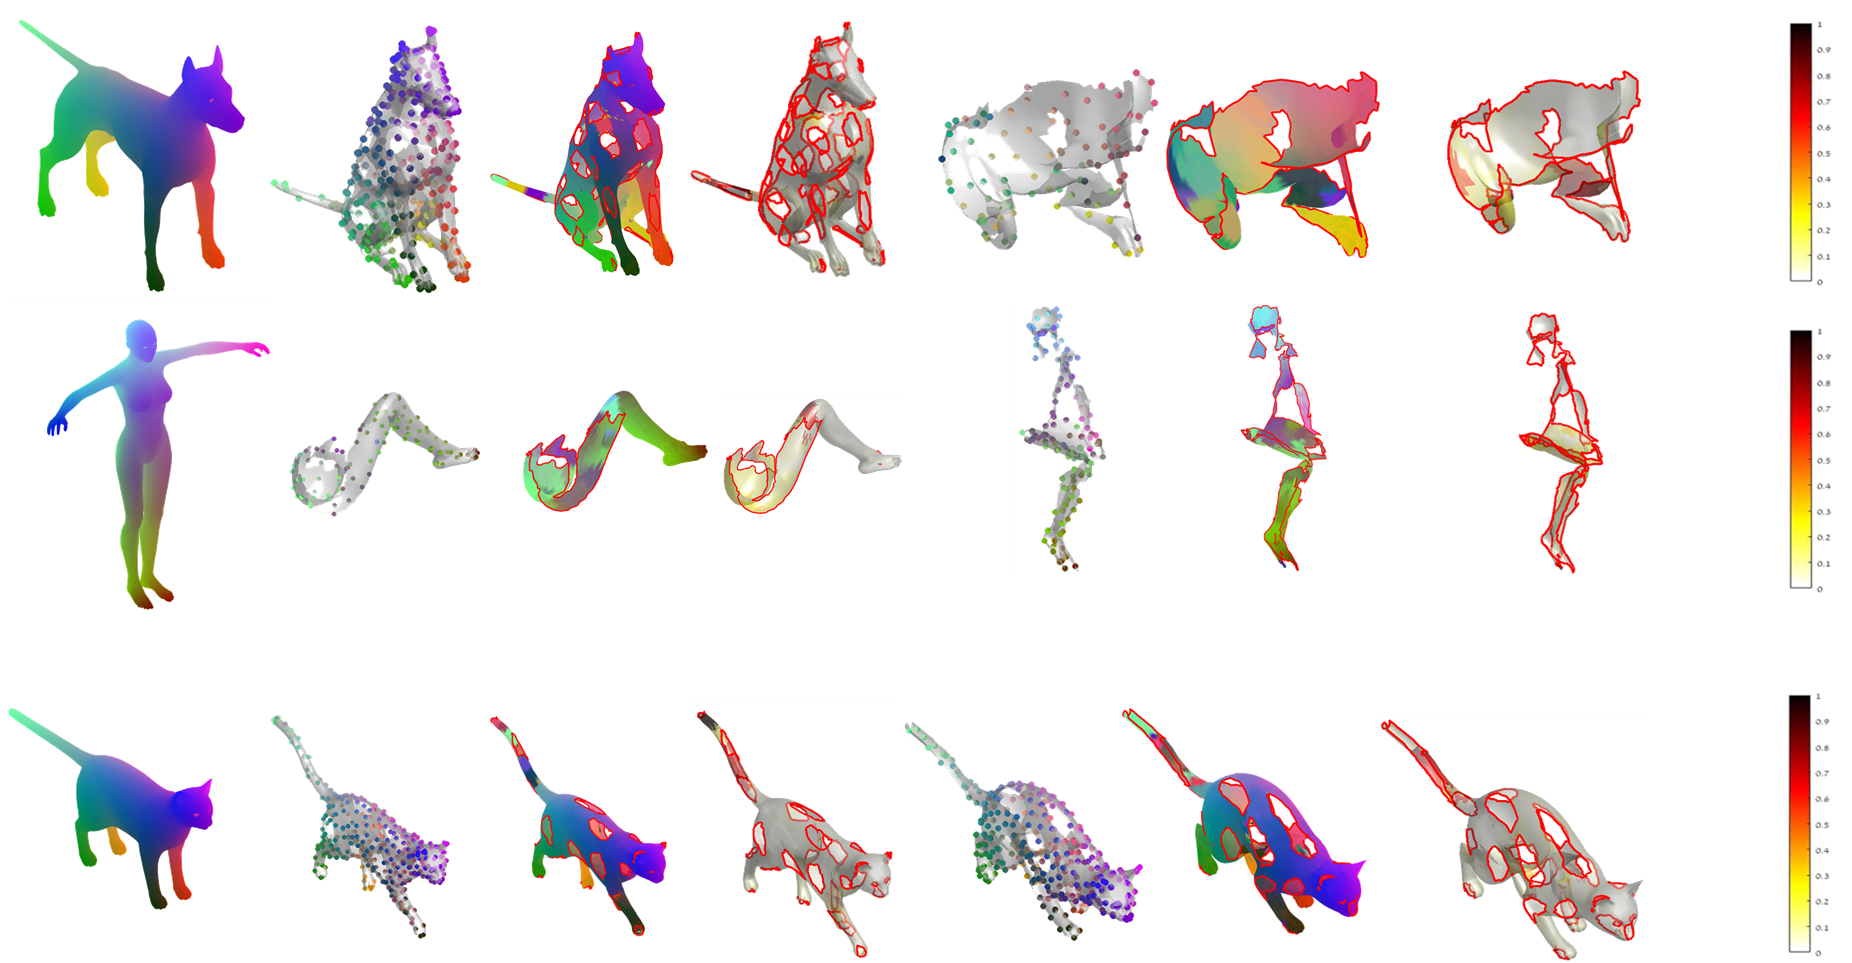
\includegraphics[width=1\textwidth]{figures/fail2.png}
	\caption{Some notable failure cases}
\end{figure*}

\paragraph{implementation}
Our code which produces the sparse correspondences is implemented entirely in C++ using the Point Cloud Library. For geodesics we have used  Fast Marching Geodesics adapted from the code published by Ron Kimmel to run in parallel on multiple cores. We calculate FPFH using $R_{FPFH}=0.03\cdot \sqrt{Area(\mathcal{M})}$, and NNF using FLANN. The average runtime on i7-4790 for 2 surfaces of ~12000 vertices is 150s.

{\small
	\bibliographystyle{ieee}
	\bibliography{egbib}
}
\end{document}